\section{System Infrastructure}
\label{sec:infra_improvements}

This section describes the core infrastructure changes that address the three highest-priority challenges identified in Chapter~3: recommendation quality, search latency, and multilingual support.
Figure~\ref{fig:new_system_overview} shows the revised architecture.

\begin{figure}[H]
\centering
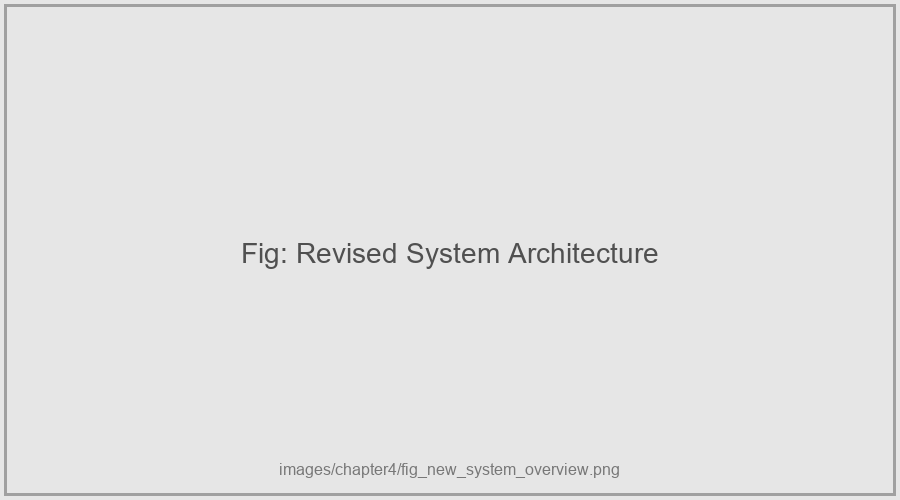
\includegraphics[width=0.92\textwidth]{images/chapter4/fig_new_system_overview}
\caption{Revised system architecture. The primary changes relative to the prior system are the BGE-M3 HNSW text index, the NLLB-200 translation stage, and the dual-mode Cleora + DIF-SASRec recommendation backend.}
\label{fig:new_system_overview}
\end{figure}

\subsection{Text Encoder Upgrade: BLaIR to BGE-M3}
\label{sec:encoder_upgrade}

The BLaIR encoder is replaced by \texttt{BAAI/bge-m3}~\cite{chen2024bge}, a multilingual model producing 1{,}024-dimensional embeddings.
BGE-M3 is set as the single source of truth for all text embeddings in the system: user profile vectors, item embeddings in the FAISS text index, and query encodings at search time all use the same model, ensuring consistency across the retrieval pipeline.
The \texttt{TEXT\_EMBED\_DIM} constant in \texttt{app/config.py} is the sole location that needs updating if a future encoder is adopted.

\subsection{NLLB-200 Multilingual Translation Pipeline}
\label{sec:nllb_pipeline}

A three-stage translation pipeline is inserted before the BGE-M3 encoding step in the search route (Figure~\ref{fig:translation_pipeline}).

\begin{figure}[H]
\centering
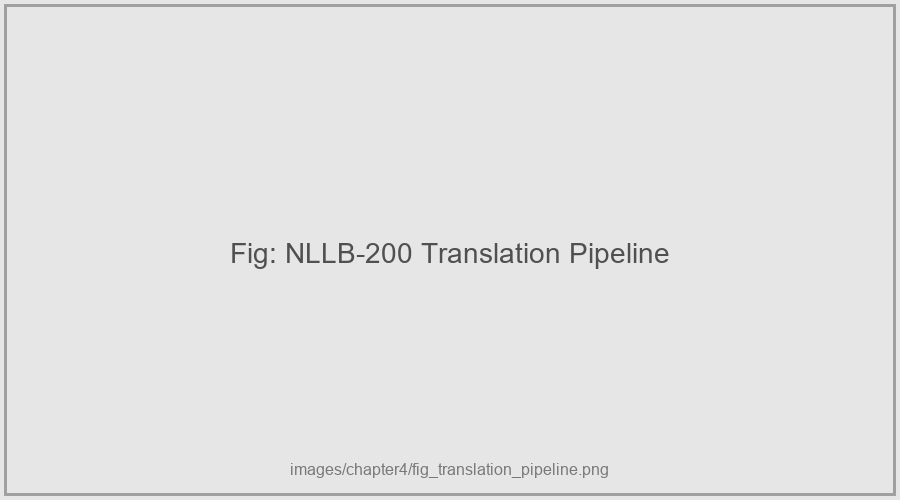
\includegraphics[width=0.88\textwidth]{images/chapter4/fig_translation_pipeline}
\caption{NLLB-200 translation pipeline. Language detection (lingua, $< 1$\,ms), greedy translation, and a quality gate that retries with beam search if the first pass leaves source-language tokens in the output.}
\label{fig:translation_pipeline}
\end{figure}

\begin{enumerate}
    \item \textbf{Language detection}: The \texttt{lingua} library identifies the input language in under 1\,ms. If the detected language is English, the translation step is skipped entirely.
    \item \textbf{NLLB-200 translation}: For the 19 supported non-English languages, the \texttt{facebook/nllb-200-distilled-600M} model translates the query to English. A fast greedy pass (\texttt{num\_beams=1}) is executed first.
    \item \textbf{Quality gate}: A heuristic checks whether any source-language words survived into the translation output — a reliable indicator of partial decoding failure. If untranslated tokens are detected, the query is retried with \texttt{num\_beams=4}, trading \textasciitilde{}30 ms for a cleaner translation.
    \item \textbf{LRU caching}: Translated queries are cached via \texttt{@lru\_cache(maxsize=2048)}, so repeated queries (e.g., common search terms) cost 0 ms after the first miss.
\end{enumerate}

Both the NLLB model and the lingua detector are lazy-loaded on first use and eagerly warmed up at server startup to eliminate the cold-start P95 latency spike.

\subsection{Search Pipeline Parallelisation}
\label{sec:parallel_search}

In the prior system, text encoding and CLIP image encoding were executed sequentially.
The revised search route runs them concurrently using an \texttt{anyio} task group:

\begin{itemize}
    \item \texttt{encode\_text\_task}: runs \texttt{ml.encode\_text(query, text\_encoder)} in a background thread.
    \item \texttt{encode\_image\_task}: runs \texttt{ml.encode\_image\_b64(..., clip\_model)} in a parallel thread.
\end{itemize}

Both tasks are submitted to the task group simultaneously; the route waits only for the slower of the two before proceeding to the FAISS and Tantivy retrieval stages.
For text-only queries, the CLIP task is skipped.
The combined effect of the encoder upgrade, HNSW index, and parallelisation reduces end-to-end warm-cache search latency from 1{,}102 ms to 59 ms — an 18.6$\times$ improvement (Table~\ref{tab:latency_stages}).

\subsection{Dual-Mode Recommendation Architecture}
\label{sec:dual_mode_rec}

The GRU-SeqDQN recommendation module is replaced by a two-pipeline architecture mapped to two distinct UI panels: \textit{People Also Buy} (Pipeline~A) and \textit{You Might Like} (Pipeline~B).
Figure~\ref{fig:rec_funnel} illustrates the recommendation funnel.

\begin{figure}[H]
\centering
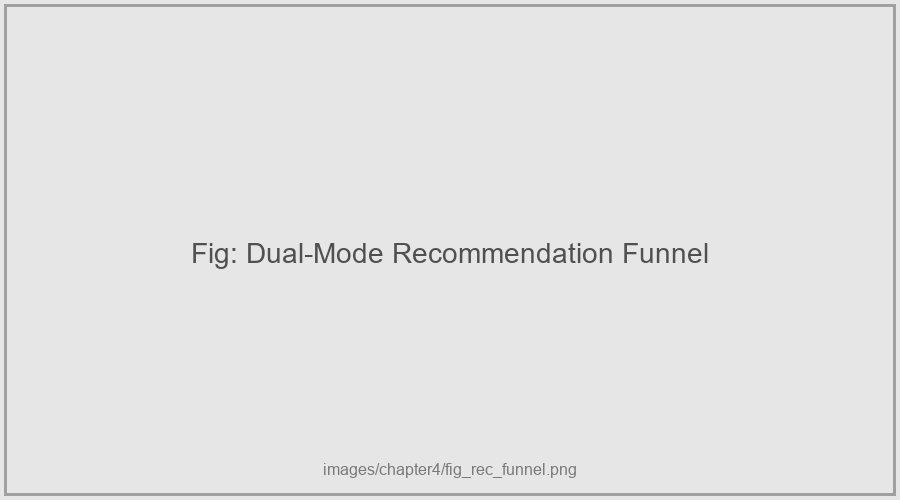
\includegraphics[width=0.90\textwidth]{images/chapter4/fig_rec_funnel}
\caption{Dual-mode recommendation funnel. Pipeline~A (behavioural) and Pipeline~B (sequential) run independently and serve distinct UI panels. Cold-start users (fewer than 5 interactions) receive items sampled from the Cleora catalogue.}
\label{fig:rec_funnel}
\end{figure}

\paragraph{Pipeline A — Cleora + BGE-M3 (People Also Buy) —}
A mean-pool of the user's interaction history is computed over BGE-M3 item embeddings to form a profile vector.
The Cleora co-purchase graph embedding index (375{,}280 items) is searched for the 50 nearest neighbours by inner product.
These candidates are then re-ranked by cosine similarity to the profile vector and the top items are returned.

\paragraph{Pipeline B — DIF-SASRec (You Might Like) —}
An \texttt{AgentPool} of 8 isolated DIF-SASRec agents handles concurrent personalisation requests.
Each agent loads the per-user checkpoint from disk, runs inference over the user's recent interaction sequence, and applies the content veto filter ($\tau = 0.3$ cosine threshold) to remove semantically unrelated candidates.
Per-user online fine-tuning is triggered at every click or cart interaction, updating the personal checkpoint via a Bellman-error training step.

\paragraph{Cold-start handling —}
Users with fewer than \texttt{COLD\_START\_THRESHOLD} = 5 interactions bypass both pipelines.
The fallback samples items uniformly from the intersection of the Cleora ASIN set and the FAISS index, providing a diverse starting point until enough signal accumulates.

